\subsection{SEARCH (64)}

Central part of the search request recursive propagation sequence. 
\textit{SearchId} is an unique randomly generated number. \textit{Public Key} 
is the 1024-bit RSA public key of the search initiatior. \textit{AHash} is the 
identifier of the file to be searched for. It is the concatenation of the 
SHA-3-512 of the file content and the SHA-3-224 of the file name concatenated 
with the textual representation of the file size. A node receiving this message 
should remember (for a limited, implementation defined time) the SearchId along 
with address of the node from where it came. This information is vital for 
forwarding potential OFFER messages to the right peers. It is also useful for 
ignoring other SEARCH messages with the same SearchId - this prevents search 
cycles. The reply contains the number of peers to which the message will be 
forwarded on the next hop, i.e. the number of neighbors minus one. For now, 
this number is not used for anything, but it might be in the future (for blind 
alley notifications for example).

\begin{figure}[H]
    \centering
    \scalebox{.33}{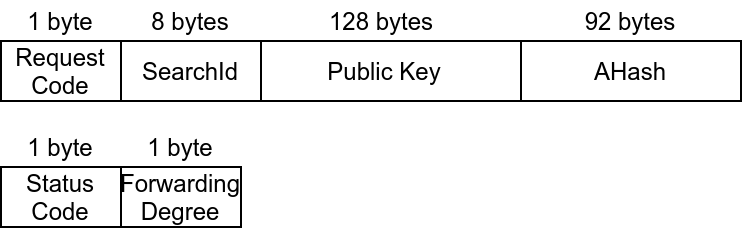
\includegraphics{figures/search}}
\end{figure}

\subsection{OFFER (65)}

This message is initiated by a peer willing to provide a file requested by the 
means of a SEARCH message. It is also propagated recursively, but directly 
through the succesful search path, without branching out to all neighbors. This 
is achieved by using the stored SearchId and request source by each node in the 
respective search path. Propagation stops when this message receives the search 
initiator.

The message itself contains the related SearchId and another randomly generated 
unique number, called \textit{OfferId}. The rest of the message contains 
information encrypted using the Public Key contained in the SEARCH message. 
OfferId will be subsequently used for facilitating the established 
communication between the search initiator and the offer initiator, which are 
completely unknown to each other. In order for this to work correctly, each 
node that this message passes through has to remember the OfferId along with 
the address of the local source. Another use for OfferId is to uniquely 
identify the file transfer between them. The encrypted part of the message 
contains a transfer key and a list of part data structures used for the actual 
file transfer and are therefore discussed in the section detailing file 
transfers.

A useful feature of file searching is the path caching mechanisms, in which 
multiple peers collectively remember a the network path to the provider of a 
certain file. Multiple paths can exist for the same file. No single node knows 
the whole path, they just cache the addresses of the next hops for a given 
AHash. A future SEARCH request for this AHash will be forwarded just through 
the cached paths, instead of branching out to all local neighbors.

The reply for this message does not have any data besides the status code.

\begin{figure}[H]
    \centering
    \scalebox{.33}{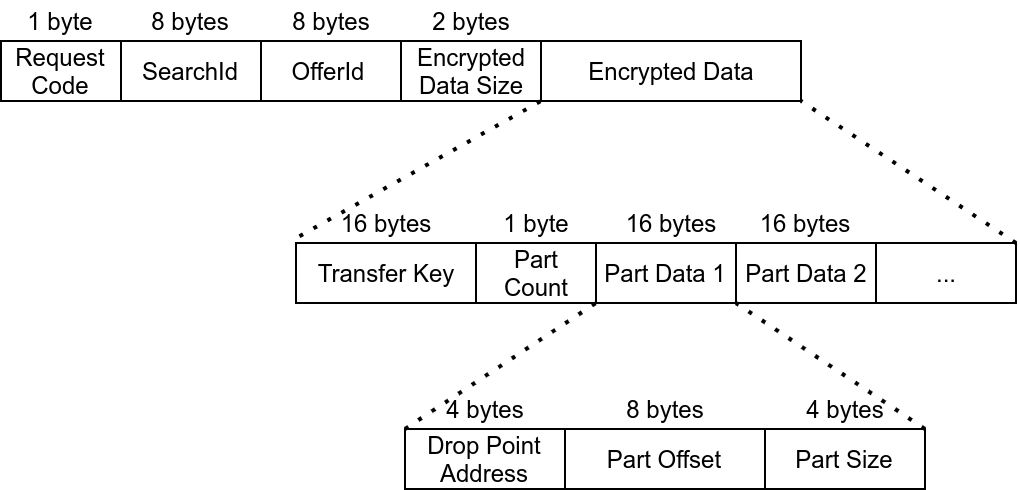
\includegraphics{figures/offer}}
\end{figure}

\subsection{UNCACHE (66)}

In the unfortunate and inevitable event that a peer which is part of a cached 
search path leaves the network, the part of the path up to the current node is 
left invalidated. There needs to be some kind of mechanism for notifying the 
previous node that the next hop is no longer alive. The UNCACHE command does 
just that. It is propagated backwards through the cached path which was 
invalidated, so the peers can remove the path information from their local 
cache. The reply for this message does not have any data besides the status 
code.

\begin{figure}[H]
    \centering
    \scalebox{.33}{
\includegraphics{figures/uncache}}
\end{figure}

\subsection{CONFIRMTRANSFER (67)}

This message is initiated by the same peer which initiated the search request. 
It is propagated backwards through the same path which was followed by the 
related OFFER message. It leverages the stored information on each node to find 
its way to the offer initiator, along with the OfferId parameter in the message 
data. When the offer initiator receives this message, it starts the file 
transfer process. The reply for this message does not have any data besides the 
status code.

\begin{figure}[H]
    \centering
    \scalebox{.33}{
\includegraphics{figures/confirmtransfer}}
\end{figure}
